将词包作为文本的特征是一个经典,简单直观而有效的特征提取方式,课上也讲过这个方法。
在词包模型中,文本被表示成组成它的词的包(多重集合)。
这个集合保留了词的重复次数,但是忽略文本的语法和词之间的顺序。\\
词包模型首先构建文本的词汇表,然后取最频繁的词汇作为词包的考察元素。
对于每个文本,统计各个频繁词的出现次数,作为该段文本的特征。\\
举例来讲,我们有两段文本:
\begin{itemize}
	\item
	  ``John likes to watch movies. Mary likes movie too.''
	\item
	  ``John also likes to watch football games.''
\end{itemize}
由这两段文本构造的词包为:
[ "John", "likes", "to", "watch", "movies", "also", "football", "games", "Mary", "too"]。
有了词包之后,我们就可以来构造文本的特征了。
最常用的方式是词汇频数。
上述例子构造的文本特征为:
\begin{itemize}
	\item
	  ``[1, 2, 1, 1, 2, 0, 0, 0, 1, 1]''
	\item
	  ``[1, 1, 1, 1, 0, 1, 1, 1, 0, 0]''
\end{itemize}

\subsubsection{简单词包}
我们采用scikit-learn提供的词包模块(sklearn.feature\_extraction.text.CountVectorizer)来计算文本的词包特征。\\
我们抽出训练集词包中的前几个词: ['abandoned',
'abc',
'abilities',
'ability',
'able',
'abraham',
'absence',
'absent',
'absolute',
'absolutely'
]。\\

提取出特征后,使用了三种分类器:
\begin{itemize}
	\item
	  随机森林模型  \\
	  (sklearn.ensemble.RandomForestClassifier)
	\item
	  高斯朴素贝叶斯模型  \\
	  (sklearn.naive\_bayes.GaussianNB)
	\item
	  线性回归模型  \\
	  (sklearn.linear\_model.LogisticRegression)
\end{itemize}
三种分类器的分类结果如下图所示(图\ref{fig:rfroc}, 图\ref{fig:gnbroc}, 图\ref{fig:lrroc}, 图\ref{fig:3croc}),我们以ROC和AUC作为评价结果。
\begin{figure}[h]
\centering
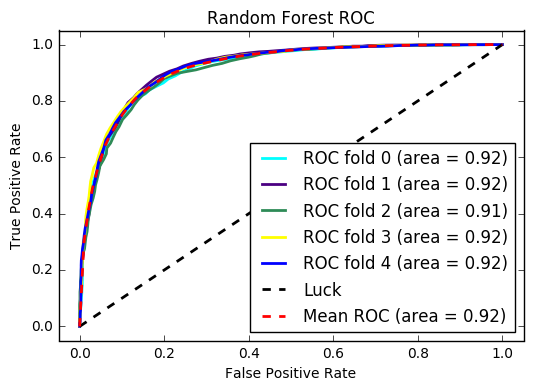
\includegraphics[width=0.9\linewidth]{rf_roc}
\caption[rf_roc]{随机森林模型交叉验证的ROC曲线}
\label{fig:rfroc}
\end{figure}

\begin{figure}[p]
\centering
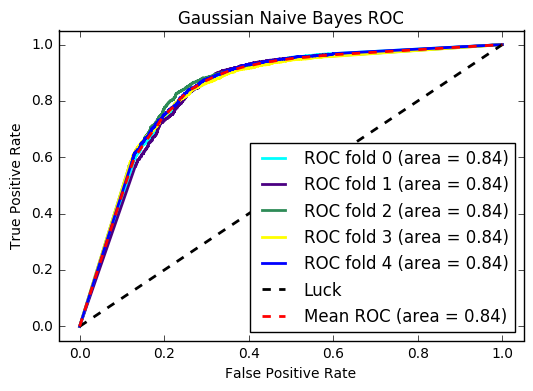
\includegraphics[width=0.9\linewidth]{gnb_roc}
\caption[gnb_roc]{高斯朴素贝叶斯模型交叉验证的ROC曲线}
\label{fig:gnbroc}
\end{figure}

\begin{figure}[p]
\centering
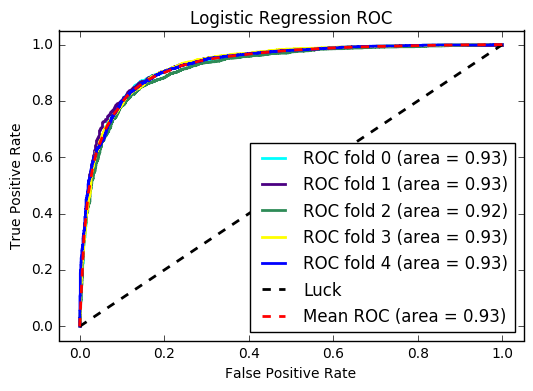
\includegraphics[width=0.9\linewidth]{lr_roc}
\caption[lr_roc]{线性回归模型交叉验证的ROC曲线}
\label{fig:lrroc}
\end{figure}

\begin{figure}[p]
\centering
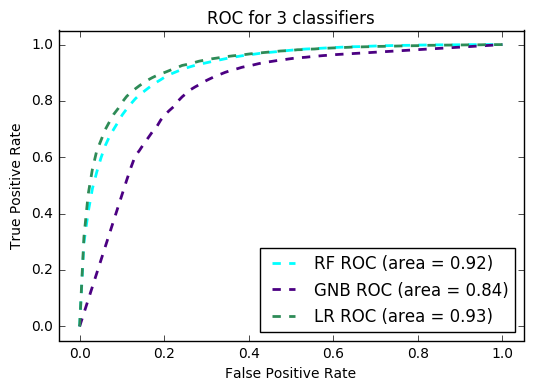
\includegraphics[width=0.9\linewidth]{3c_roc}
\caption[3c_roc]{三种模型的平均ROC曲线}
\label{fig:3croc}
\end{figure}

从三种分类器的K次交叉验证绘制出的ROC曲线来看,各个交叉验证集的ROC曲线几乎完全重合,似乎没有必要对这个数据集进行交叉验证。
另一方面,我们在实验中使用了5次交叉验证,也就是说训练时间比单个训练集测试集的方式多了4倍。
从性能和运行效率的角度考虑,我们在之后的实验中不再进行交叉验证,以节省时间。\\
在三种分类模型的横向比较中,我们发现训练过程中,随机森林的训练时间 > > 线性回归模型 > 高斯朴素贝叶斯模型。
而随机森林模型和线性回归模型的分类性能相差不大。
\paragraph{简单词包的问题}